\section{Agile Methoden und Open Source}
(Autor: Henn)\\

Der große Hype um agile Methoden ist bereits vorüber. Doch haben agile Methoden die herkömmliche Softwareentwicklung nachhaltig beeinflusst. Die Fachzeitschriften sind voll davon und in Firmen werden agile Vorgehensweisen immer häufiger umgesetzt. Doch wie sieht die Situation in Open Source Projekten mit ganz anderen Umständen und Herausforderungen aus?

In diesem Abschnitt wird ein Blick in die Open Source Welt geworfen und analysiert, inwiefern agile Techniken eingesetzt werden. Im Anschluss werden Chancen und Probleme bei der Verwendung eines agilen Modells im Open Source Bereich dargestellt.

\subsection{Open Source Projekte}
Bei der Recherche fiel auf, dass es gar nicht so leicht ist, Open Source Projekte zu finden, die von sich selbst behaupten, sie würden nach agilen Vorgehensmodellen vorgehen. Allerdings finden sich auch in anderen Projekten Techniken, die eindeutig aus der agilen Softwareentwicklung stammen. Im Folgenden sollen einige Projekte als Stellvertreter für verschiedene Stufen der Adaption mit Blick auf die Umsetzung agiler Techniken und Prinzipien betrachtet werden.

\subsubsection{TYPO3}
Die Entwickler des Open Source Content Management Systems TYPO3 haben sich dazu entschieden, ihre nächste Version, TYPO3 5 (Phoenix) vollständig nach dem Scrum Vorgehensmodell  (Siehe Kapitel \ref{ch:scrum}) zu entwickeln. Anhand dieses Beispiels soll gezeigt werden, wie es möglich ist, ein solches Vorgehensmodell im Open Source Bereich vollständig umzusetzen und was es für Bedingungen gibt, damit dies erfolgreich geschehen kann.
\begin{figure}[h]
	\centering
	
\includegraphics[width=0.5\textwidth]{images/typo3_Phoenix_logo.jpg}
	\caption{Logo TYPO3 5.0 Phoenix\cite{bib:phoenix-logo}}
	\label{Logo-Phoenix}
\end{figure}

Ein Sprint dauert beim TYPO3 Phoenix Team 4 Wochen. Innerhalb dieses Sprints finden tägliche Meetings statt und am Ende eines Sprints muss eine lauffähige Version bereit stehen. Abbildung \ref{magic-cycle} visualisiert diesen Zyklus. User Stories aus dem Product Backlog werden für diesen Sprint ausgesucht und in einem Sprint Backlog festgehalten. Diese Stories werden dann innerhalb der 2-4 Wochen implementiert.
\begin{figure}[h]
	\centering
	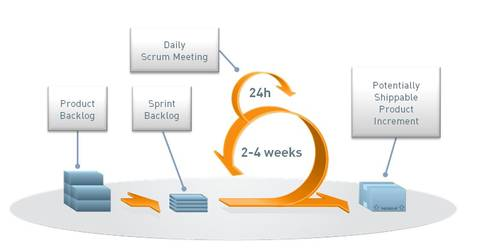
\includegraphics[width=1\textwidth]{images/typo3-magic-cycle.jpg}
	\caption{Magic Cycle - TYPO3 Scrum Implementierung\cite{bib:agiler-phoenix}}
	\label{magic-cycle}
\end{figure}

Als Product-Owner, der im klassischen Scrum aus einer Person besteht, wurde für Phoenix  ein kleines Team bestehend aus drei Personen eingerichtet. Dies erscheint sinnvoll, da es sich bei Phoenix um eine Gemeinschaftsentwicklung handelt. Eine einzelne Person als Product-Owner würde dem Community Gedanken entgegen wirken und  wäre darüber hinaus wahrscheinlich auch noch überlastet, wenn sie plant, diese Aufgabe in ihrer Freizeit auszufüllen. Diese drei Personen diskutieren über die Features, die innerhalb eines Sprints implementiert werden sollen und priorisieren diese\cite{bib:forge}.

Die Rolle des Scrum-Masters wird wiederum nur von einer Person besetzt. Hier würden sich zwei oder mehr Scrum Master eher gegenseitig bei der Leitung von Gesprächen behindern. Außerdem ist die Aufgabe des Scrum Masters nicht so fordernd und aufwändig, wie die des Product Owners. Sollte die Person, die die Rolle des Scrum Masters inne hat zwischenzeitlich ausfallen, so wäre es auch nicht allzu schwierig, sie kurzfristig zu ersetzen\cite{bib:forge}.

Das eigentliche Scrum-Team für die Phoenix Entwicklung besteht aus 19 Entwicklern\cite{bib:forge}, die alle miteinander in Kontakt stehen und koordiniert werden müssen. Entscheidend für den Erfolg von Scrum im Phoenix Team ist daher das Internet. Es bietet vielfältige Möglichkeiten, miteinander zu kommunizieren und große räumliche Entfernungen zu überbrücken. So kommuniziert das Team:
\begin{itemize}
\item Sprint-Planung, Review und Retrospektive werden durch Meetings im Internet durchgeführt.
\item Es steht ein Jabber Chatroom bereit, in dem sich das Team kurzfristig abstimmen kann und Fragen während der Entwicklung geklärt werden können.
\item jeden Tag findet um 17:00 Uhr das Daily Scrum Meeting mittels Webex oder Skype statt. Danach wird das Protokoll der Sitzung über die Mailing Liste verschickt, damit alle, die nicht teilnehmen konnten, trotzdem auf dem neusten Stand sind.
\item Das Sprint-Backlog wird ebenfalls im Internet unter forge.typo3.org\cite{bib:forge} gepflegt.
\item TYPO3 Veranstaltungen werden so oft, wie möglich genutzt um persönlich miteinander sprechen zu können
\item Nach jedem Sprint wird das Ergebnis sowohl als Nachricht, als auch als laufende Demo-Installation bekanntgegeben\cite{bib:agiler-phoenix}
\end{itemize}

\begin{figure}[h]
	\centering
	\fbox{
		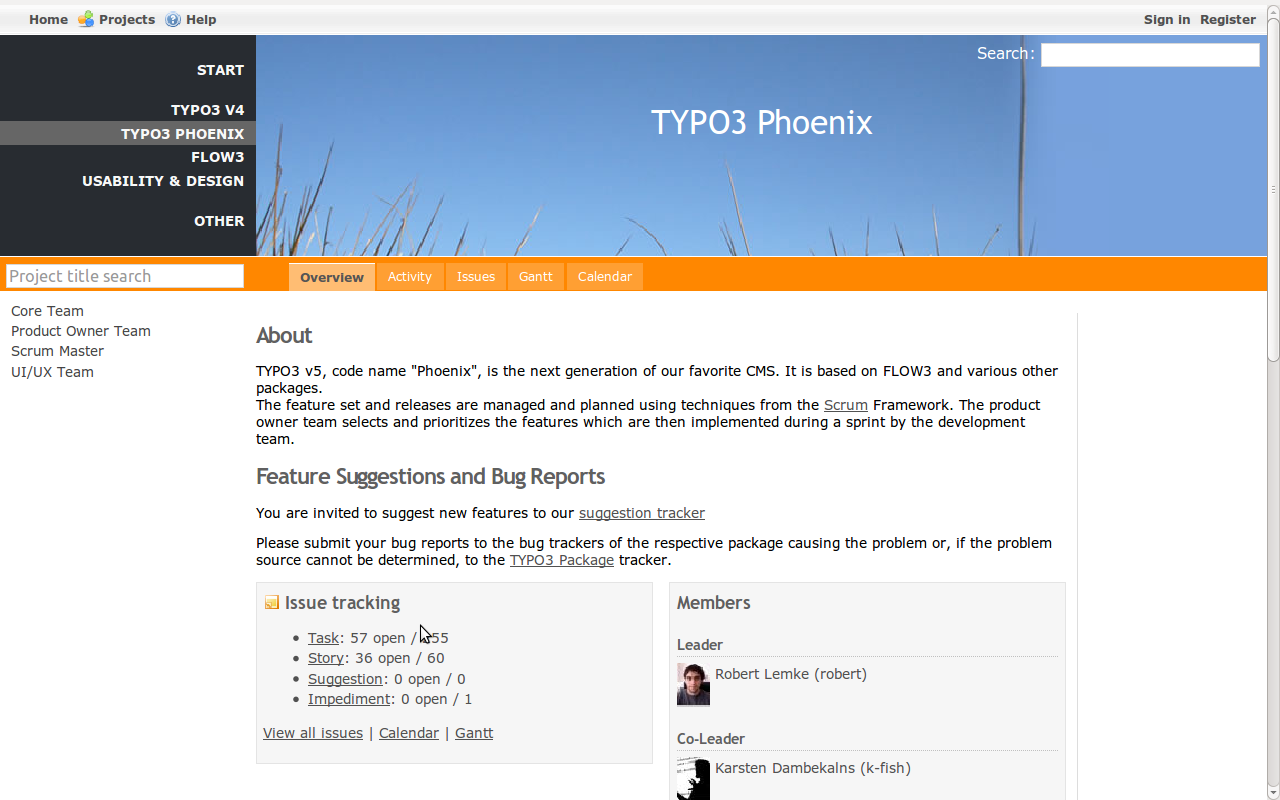
\includegraphics[width=1\textwidth]{images/forge-typo3-org.png}
	}
	\caption{forge.typo3.org\cite{bib:forge}}
	\label{forge}
\end{figure}
Der gesamte Fortschritt sowie die offizielle Dokumentation und Kommunikation wird über die Web-Plattform forge.typo3.org dargestellt. Auf diese Weise ist der Entwicklungsprozess sehr transparent und für die Community einsehbar\cite{bib:scrumify}. Dadurch verliert die Entwicklung nicht an Akzeptanz.

Auf der Website des Phoenix Teams wurden mehrere Bereiche eingerichtet:
\begin{description}

\item [Core Team] Hier befinden sich alle Informationen, die das Entwicklungsteam zur Koordination benötigt. der Bereich beinhaltet
\begin{itemize}
\item eine Übersicht mit Link zum Issue-Tracker und einer Liste der Teammitglieder
\item Eine Auflistung aller bisher ausgeführten Aktivitäten, wie Wiki Änderungen, oder auch Änderungen am Quellcode
\item Eine Roadmap für den aktuellen Sprint, mit Auflistung aller in diesem Sprint zu erledigenden User Stories und den dazugehörigen Tasks
\item den Issue Tracker
\item das Sprint, sowie das Product Backlog
\item ein Gantt Chart
\item ein Kalender
\item  ein Wiki
\item das Repository mit dem Quellcode
\end{itemize}

Das Wiki beinhaltet alle wichtigen Informationen für Entwickler, sowie teilweise Erklärungen zum Scrum Prozess und Richtlinien.  So findet sich dort zum Beispiel die Erklärung, was es mit der ''Definition of Done``  auf sich hat, die bei Scrum ein wichtiges Artefakt darstellt.

\item [Product Owner Team] Für das Product Owner Team gibt es ebenfalls wie beim Core Team eine Übersicht mit den Mitgliedern, sowie eine kurze Beschreibung der Gründe, sich für ein Teams als Product Owner zu entscheiden. Es finden sich ebenso Übersichten über Aktivitäten, Issues und Termine. Außerdem wird ebenfalls ein Wiki gepflegt. Dieses Wiki beschäftigt sich   allerdings viel stärker mit dem Scrum Entwicklungsprozess, als das Wiki des Core Teams. So ist hier der eigentliche Entwicklungsprozess für TYPO3 Phoenix beschrieben, sowie für alle, die Scrum noch nicht so intuitiv leben ein kleines Cheat Sheet hinterlegt, das den Scrum Prozess nochmals auf einer Seite übersichtlich zusammenfasst. Ebenso findet sich hier eine Liste mit Benutzerrollen für TYPO3. Im Anschluss daran sind die Protokolle der einzelnen Scrum Meetings hinterlegt.

\item [Scrum Master] im Bereich des Scrum Masters gibt es lediglich eine Übersicht, einen Bereich, in dem die Aktivitäten aufgelistet werden, sowie Issue Tracker, Gantt Chart und ein Kalender. Da die Rolle des Scrum Masters nur durch eine Person besetzt ist, wird hier auch nicht mehr Inhalt benötigt.

\item [UI/UX Team] dieses Team beschäftigt sich mit dem User Interface, sowie der User Experience. Es finden sich die Übersichten, über Issues und Aktivitäten, wie in den anderen Bereichen. Auf den Scrum Prozess wird hier nicht weiter eingegangen. \cite{bib:forge}
\end{description}


Die TYPO3 Entwickler haben es geschafft, den gesamten Scrum Prozess mit minimalen Anpassungen hinsichtlich räumlicher Entfernungen, für ihr Projekt zu adaptieren. Von entscheidendem Vorteil für die TYPO3 Entwickler, ist die Tatsache, dass sie alle aus Deutschland kommen. So ist es deutlich einfacher, einen Termin, der auf 17:00 Uhr angesetzt wurde, auch wahrzunehmen. Eine solche regelmäßige zeitliche Abstimmung würde bei Entwicklern, die über die ganze Welt verstreut leben nicht funktionieren. Außerdem ist es so für die Projektteilnehmer leichter, zu den TYPO3 Veranstaltungen zu fahren, da diese ebenfalls hauptsächlich in Deutschland stattfinden. Auch hier wäre es für einen weit verstreutes Entwicklerteam zeitlich, als auch  finanziell nicht möglich, sich so oft persönlich zu sehen. Ein weiterer Faktor ist sicherlich die Größe des Projektteams. Bei nur 17 Mitgliedern ist es leichter möglich,die Koordination über das Internet zu  organisieren und dafür zu sorgen, dass auch wirklich alle gerade aktiv am Projekt teilnehmen können.

\subsubsection{Firefox}
Das Firefox Projekt besteht aus zahlreichen Unterprojekten. Diese gehen teilweise sehr unterschiedlich vor.
\begin{figure}[h]
	\centering
	\fbox{
		
\includegraphics[width=0.15\textwidth]{images/firefox-3.jpg}
	}
	\caption{Logo Firefox\cite{bib:logo-firefox}}
	\label{fireLogo}
\end{figure}
So ist zum Beispiel das Tracemonkey Projekt, ein Just in Time (JIT) Compiler für JavaScript äußerst agil unterwegs. Das Projekt bezeichnet sich selbst als ''in rapid development mode''\cite{bib:trm}. So ist es zum Beispiel sehr leicht, Code beizutragen. Selbst wenn dieser nicht alle Tests bestanden hat. Man muss nur erklären, warum er den Test nicht besteht und was passieren muss, um diesen Fehler zu beheben'\cite{bib:trm}. Voraussetzung ist allerdings, dass man im Anschluss daran erreichbar ist. Dies deutet auf eine Art der Entwicklung hin,  bei der Vieles durch schnelle und direkte Kommunikation ausgemacht wird und das Team sehr flexibel und gemeinschaftlich am Quellcode arbeitet.  Ein Vertreter der traditionellen Entwicklung ist beispielsweise das  Compositor Projekt, das  Teil der Rendering Engine Gecko ist \cite{bib:beltzner}.

Mit der Version 4 des Firefox wurde ein neues Entwicklungsmodell eingeführt. Dies soll den Missstand beheben, dass es sehr lange dauert, bis eine neue Version des Firefox herausgegeben wird, die auch wirklich neue Features mit sich bringt. Ein Umstand, der die Motivation der Entwickler nicht gerade fördert, da neue von ihnen bereitgestellte Funktionen erst ein halbes bis dreiviertel Jahr später in einer Firefox Version zur Verfügung stehen. Außerdem ist der Firefox dadurch nicht so häufig in den Medien wie andere Browser, die öfters neue Funktionalitäten bereitstellen.

Das neue Entwicklungsmodell soll die diversen Unterprojekte allerdings nicht in ihren eigenen Entwicklungsmodellen einschränken. Firefox Produkt Manager Mike Beltzner beschreibt dies wie folgt: ''Really, we're not tied to any specific development model, [...] We're tied to what is effective''\cite{bib:beltzner}. Nachfolgend soll dieses Entwickllungsmodell beschrieben werden und analysiert werden, inwieweit hier agile Prinzipien verfolgt werden.

Das neue Entwicklungsmodell sieht mehrere Entwicklungszweige vor, die pa\-ra\-llel geführt werden.
\begin{itemize}
\item mozilla-central
\item firefox-experimental (fx-exp)
\item firefox-beta (fx-beta)
\item Firefox
\end{itemize}
\begin{figure}[h]
	\centering
	\fbox{
		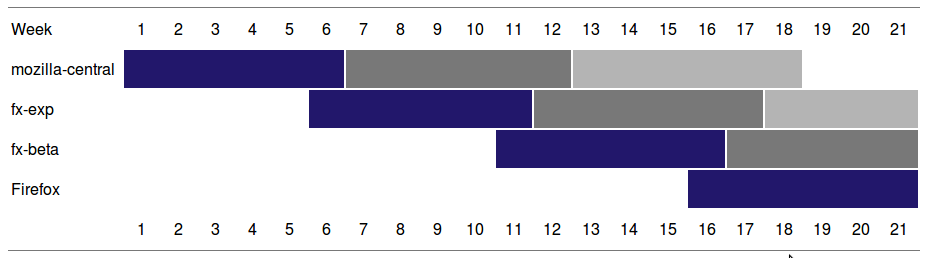
\includegraphics[width=1\textwidth]{images/timetable-firefox.png}
	}
	\caption{Zeitplan Firefox\cite{bib:fire-development}}
	\label{firett}
\end{figure}

Der Zweig mozilla-central stellt die Basis dar, in der die neusten Funktionalitäten entwickelt werden. jeweils im sechs Wochen Rhythmus werden diese Funktionalitäten, soweit sie reif genug sind in den nächst höheren Zweig überführt und dort weiter verbessert und stabilisiert, während im mozilla-central Zweig bereits an den nächsten Features gearbeitet wird. Dort besteht dann ebenfalls jeweils im sechs Wochen Rhythmus die Möglichkeit, neuen Code in den nächst höheren Zweig zu übertragen. So ist es in eingeschwungenem Zustand theoretisch möglich,  alle sechs Wochen eine neue Version des Firefox herauszugeben. Abbildung \ref{firett} zeigt den offiziellen Zeitplan des Firefox Projektes. der diesen sechs Wochen Rhythmus darstellt. Wie Abbildung \ref{fireusers} zeigt, stellen die verschiedenen Zweige außerdem eine neue Stufe des Testens dar. So soll sich die Zahl der Nutzer mit jedem Zweig verzehnfachen, um am Ende ein breit getestetes Produkt zur Verfügung stellen zu können.

Durch diese Umgestaltung ist es dem Firefox Team möglich, schnell neue Features in die offizielle Version zu bringen, ohne dass die einzelnen Unterprojekte dadurch ausgebremst werden. Teams, die traditionell entwickeln, können einfach mehrere Zyklen für sich in Anspruch nehmen und ihre Erweiterungen zu einem späteren Zeitpunkt in die nächst höheren Zweige überführen, Teams, die eher agil vorgehen werden diesen schnellen Release Zyklus nutzen und ihre neuste Version einbringen, ohne auf langsamere Projekte warten zu müssen.

\begin{figure}[h]
	\centering
	\fbox{
		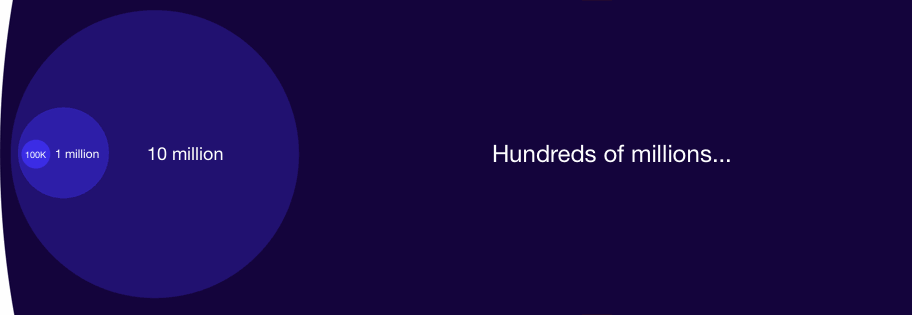
\includegraphics[width=1\textwidth]{images/firefox-channels-users.png}
	}
	\caption{Anzahl der Nutzer der in den verschiedenen Entwicklungszweigen\cite{bib:fire-development}}
	\label{fireusers}
\end{figure}

Mit der agilen Softwareentwicklung wurden schnelle Release Zyklen eingeführt. Man erhoffte sich davon einen allgemein stabileren Code, ein lebendigeres Mitarbeiten und eine erhöhte Flexibilität, was Änderungen der Anforderungen betrifft. Das Entwicklungsmodell des Firefox Teams orientiert sich an diesen Gedanken, ohne jedoch alle Entwickler dazu zu zwingen, nun nach einem agilen Entwicklungsmodell vorzugehen. Ein solch schneller Release Zyklus macht allerdings nur Sinn, wenn ausreichend Entwickler vorhanden sind, die in kurzen Zyklen neue Funktionalitäten bereitstellen.

Zusammengefasst lässt sich sagen, dass aufgrund vieler negativer Aspekte des bisherigen Entwicklungsprozesses das Firefox Team eine agilere Vorgehensweise eingeführt hat, die es ermöglicht deutlich schneller Funktionalität zu implementieren und zu veröffentlichen. Dadurch wird die Motivation der Entwickler gesteigert, da sie schneller in den Genuss der Auswirkungen ihres Schaffens kommen. Aufgrund der Tatsache, dass sich diese oft hobbymäßig dazu entschließen, an Open Source Projekten mitzuarbeiten, ist dies ein nicht zu unterschätzender Faktor, wie zum Beispiel das GIMP Projekt zeigt, das an erheblichem Nachwuchsmangel leidet, da neue Entwickler das Projekt zu oft demotiviert wieder verlassen,  da neue Features ewig in den Repositories lagen, ohne veröffentlicht zu werden\cite{bib:gimp}. Ein weiterer positiver Effekt ist, dass in den Medien öfters über Firefox geschrieben wird, da der Entwicklungsprozess durch ständige neue Versionen transparenter ist und häufiger über neue Funktionen berichtet werden kann. Dadurch bleibt Firefox in der Öffentlichkeit und es  wird der Eindruck erzeugt, dass dieses Projekt sehr lebendig und gesund ist. Dies erhöht den Bekanntheitsgrad und verbessert das Image. Trotz dieser Umstrukturierung wird den zahlreichen Unterprojekten auch weiterhin jegliche Freiheit gelassen, ihr favorisiertes Entwicklungsmodell weiterhin einsetzen zu können, ohne jedoch andere Projekte zu behindern.

Nachteilig ist allerdings der erhöhte Aufwand bei der Überführung der neuen Funktionen in die nächst höheren Entwicklungszweige. Dort muss viel zusammengeführt und angepasst werden, damit der Code trotzdem lauffähig bleibt. Für solche Aufgaben braucht man viele Entwickler, die sich dieser undankbaren Aufgabe annehmen. Ebenso wird eine große Anzahl an Entwicklern benötigt, die ein paralleles Entwickeln in den verschiedenen Zweigen erst ermöglichen. Das Firefox-3Team scheint aber als sehr populäres Open Source Projekt nicht an Personalmangel zu leiden.

\subsubsection{PostgreSQL}
PostgreSQL ist eine Datenbank, die in direkter Konkurrenz zu den großen Datenbanken dieser Welt, wie zum Beispiel Oracle steht\cite{bib:pg-oracle}. Bei PostgreSQL steht Sicherheit und Beständigkeit an erster Stelle.
\begin{figure}[h]
	\centering
	\fbox{
		
\includegraphics[width=0.15\textwidth]{images/logo-postgresql.png}
	}
	\caption{Logo PostgreSQL\cite{bib:pg-logo}}
	\label{pgLogo}
\end{figure}
Die Entwicklung wird hauptsächlich von Firmen getragen, die mit Post\-gre\-SQL Geld verdienen wollen\cite{bib:pg-contrib}. Erstaunlich ist, dass es auf den ersten Blick kein wirkliches Entwicklungsmodell gibt. Es gibt hauptsächlich eine umfangreiche TODO Liste, in der alle Bugs und Feature Requests aufgelistet werden\cite{bib:pg-todo}. Dort kann sich jeder Entwickler eine Aufgabe heraussuchen, die ihn anspricht und bearbeiten. Dies ist eigentlich schon ein sehr agiles Vorgehen, da auch bei agiler Softwareentwicklung die Entwickler entscheiden, was für User Stories sie als nächstes bearbeiten wollen. Allerdings sind die Einträge in der TODO Liste keine Stories, sondern einzlne Tasks die im agilen Bereich unter einer User Story stehen würden. So fehlt bei PostgreSQL ein klares Entwicklungsziel und eine Roadmap. So wird zum Beispiel festgehalten, dass im dritten Quartal 2011 möglicherweise eine neue Version erscheinen soll. Was diese neue Version allerdings für Features erfüllen muss, um veröffentlicht zu werden, wurde nirgends definiert\cite{bib:pg-roadmap}.

Dieser Umstand führt nun von außen betrachtet zu dem Schluss, dass ein Großteil der Entscheidungsfindung direkt über Chats und Mailinglisten stattfindet. Das Ergebnis dieser Entscheidungsfindung wird dann in Tasks für die TODO Liste aufgespaltet und findet sich dort als einzige offizielle Dokumentation wieder. Da sich viele bezahlte Entwickler an dem Projekt beteiligen, ist es sehr wahrscheinlich, dass genau diese dadurch einen großen Einfluss auf die Richtung des Projekts haben, da sie sich hauptberuflich mit dem Projekt beschäftigen und die meiste Zeit für solche Zieldiskussionen in Chats verfügbar sind.

Versucht man hier agile Strukturen zu erkennen, so könnte man in diese Form der Entscheidungsfindung im besten Fall durchaus agile Methoden hinein interpretieren. Da die hauptberuflichen Entwickler wohl auch die meiste Entwicklung selbst erledigen, könnte man annehmen, dass es hier ein Team von Entwicklern gibt, die täglich engen Kontakt pflegen und sehr agil über neue Anforderungen entscheiden. Allerdings ist das Entwicklungsmodell, sowie die Entscheidungen nirgends dokumentiert.

Deutet man die Indizien allerdings eher pessimistisch, so könnte man sagen, dass es bei PostgreSQL keinen wirklichen Zug hinter der Entwicklung gibt und lediglich die Entwickler aus Firmen die firmeneigenen Interessen umsetzen, während die Community nach Lust und Laune mal hier und mal da ein neues Feature hinzufügt, ohne eine richtige Idee zu haben, wohin die Entwicklung führen soll.

Die Wahrheit liegt wahrscheinlich näher an dem erstgenannten positiven Szenario, da das PostgreSQL Projekt schon sehr lange existiert und die Datenbank eine ernstzunehmende Konkurrenz für Oracle ist. Auch Entwicklungsrichtungen müssen erfolgreich kommuniziert worden sein, da PostgreSQL seine früheren Geschwindigkeitsdefizite mittlerweile aufgearbeitet hat und nun auch bei Geschwindigkeitsbenchmarks den Vergleich zu anderen Datenbanken, wie zum Beispiel MySQL nicht scheuen muss.

Zusammenfassend lässt sich sagen, dass PostgreSQL wohl ein Vertreter der traditionellen Open Source Entwicklung ist. Entscheidungen werden schnell in Chats, Mailinglisten, oder größeren Events getroffen und die Community ist ziemlich frei bei der Wahl, welches Feature als nächstes implementiert werden soll. Dies passt ganz gut zu einem agilen Vorgehensmodell. Allerdings gibt es keine festen Release Termine, sondern nur vage Andeutungen, wann vielleicht mal wieder eine neue Version erscheinen könnte. Dies wird wohl viele Open Source Entwickler abschrecken, da wieder die Gefahr besteht, dass neue Features lange unveröffentlicht in den Repositories liegen, ohne eingesetzt zu werden. Ein Motivationsproblem, das bei PostgreSQL wohl nicht so stark zum Tragen kommt, da die meisten Hauptentwickler von ihren Firmen dafür bezahlt werden, sich an PostgreSQL zu beteiligen.

Nachdem nun mehrere Open Source Projekte hinsichtlich agiler Methoden untersucht wurden, sollen nun aus den einzelnen Beobachtungen allgemeine Vor- und Nachteile agiler Softwareentwicklung im Open Source Bereich extrahiert werden.
\subsection{Vorteile agiler Methoden in Open Source Projekten}

\begin{itemize}
	\item Je agiler ein Projekt auf neue Anforderungen reagieren kann, desto schneller können Wünsche aus der Community umgesetzt werden. Dies führt zu einer motivierten Community, die viele Wünsche äußert.
	\item Entwickler, die neue Features beisteuern werden ebenfalls motiviert, da diese Features schnell in neuen Releases wiederzufinden sind.
	\item Agile Modelle legen viel Wert auf das Miteinander und das Zwischenmenschliche. Dies kann einer Community aus Freizeit Entwicklern nur gut tun.
	\item Reduzierte Dokumentation kommt den meisten Entwicklern sehr entgegen und steigert die Motivation
\end{itemize}
  
\subsection{Nachteile agiler Methoden in Open Source Projekten}
\begin{itemize}
	\item Je größer die Community wird, desto schwieriger wird die Kommunikation.
	\item Sind die Entwickler stark über die Erde verstreut, wird es schwierig mit Treffen, an denen alle Entwickler teilnehmen können
	\item Da viele Entwickler eines Open Source Projekts ausschließlich in ihrer Freizeit am Projekt mitarbeiten können, kann ein agiles Projekt mit engem Zeitrahmen und dem Bedarf der häufigen direkten Kommunikation sehr zeitintensiv sein. Freizeitentwickler könnten dadurch überfordert sein, oder sogar vom restlichen Team abgehängt werden.
\end{itemize}

  \subsection{Fazit}
  Agile Methoden passen sehr gut zu Open Source Projekten. Der Community Gedanke wird unterstützt und soziales Miteinander durch viel Kommunikation und Teamarbeit gefördert. Das TYPO3 Projekt zeigt eindrücklich, wie es möglich ist, ein Team nahezu ausschließlich über das Internet zu organisieren und das Problem der räumlichen Entfernung zu minimieren. Flexible Anpassungen der Anforderungen, sowie schnelle Release Zyklen steigern die sowohl die Motivation der Entwickler, als auch der Anwender, die Wünsche äußern, oder gefundene Bugs reporten. Allerdings ist es schwierig, eine größere Entwicklergemeinde komplett auf solche Modelle umzustellen, da die Komplexität der Koordination und der Kommunikation mit der Teamgröße sehr schnell ansteigt. Hier sei nochmals auf das Firefox Projekt hingewiesen. Es wurden Unterprojekte gegründet, die leichter zu organisieren sind und ihr Entwicklungsmodell frei wählen können, ohne andere Teams zu bremsen oder sonstig zu behindern. Das PostgreSQL Projekt zeigt, dass es auch in der traditionellen Open Source Entwicklung bereits agile Ansätze gab. Diese allerdings noch effizienter hätten ausgestaltet werden können. Aus dem PostgreSQL Projekt kann man vielleicht weiterhin ableiten, dass Projekte, die sehr stark auf Sicherheit und Stabilität fokussiert sind eher auf konventionelle Entwicklungsmodelle zurückgreifen, um sich für neue Releases ausreichend viel Zeit zu nehmen, um diese auszuhärten und zu stabilisieren. Allerdings wird auch bei einem häufig in Firmen eingesetzten Content Management System wie TYPO3 viel Wert auf Sicherheit und Stabilität gelegt. Inwieweit die neuste Version diese Anforderungen erfüllt wird sich zeigen, nachdem die erste fertige Version veröffentlicht wurde.


